\documentclass{standalone}
\usepackage{mathtools}
\usepackage{pgfplots}
\pgfplotsset{compat=1.17}
\usepgfplotslibrary{groupplots}
\begin{document}
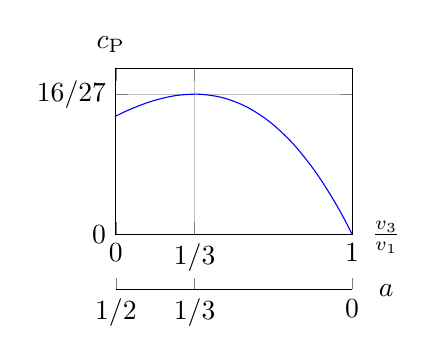
\begin{tikzpicture}
	\begin{axis}[
        x=3cm,
        xmin=0,xmax=1,
        yshift=-.7cm,
        height=2cm,
        hide y axis,
        axis x line*=bottom,
        ymin=0, ymax=1,
        xtick = {0,1/3,1},
        xticklabels={1/2,1/3,0},
        xlabel={$a$},
        xlabel style={
      yshift=22,
      xshift=55,
      anchor=north}
    ]
    \end{axis}
	
	\begin{axis}[x=3cm,y=3cm,grid=major, xmin=0, xmax=1, ymin=0, ymax=0.7, xlabel=$\frac{v_3}{v_1}$, 
	ylabel=$c_{\textnormal{P}}$,
	ytick={0,16/27},
	xtick={0,1/3,1},
	yticklabels={0,16/27},
	xticklabels={0,1/3,1},
	xlabel style={
        yshift=25,
        xshift=55,
        anchor=north},
    ylabel style={
        rotate=-90,
        yshift=45,
        xshift=30,
        anchor=north}
	]
	\plot[blue] plot[samples=100, smooth] expression{(1+x)/2*(1- x^2)};
	\end{axis}	
	\end{tikzpicture}
\end{document}